\documentclass[a4paper, 12pt]{article}
\usepackage[total={17cm,25cm}, top=2.5cm, left=2.5cm, right=2.5cm,  includefoot]{geometry}
\usepackage[utf8]{inputenc}
\usepackage{array}
\usepackage{multirow}
\usepackage{hhline}
\usepackage{gensymb}
\usepackage{graphicx}
\graphicspath{ {} }
\usepackage[czech]{babel}
\usepackage{enumitem}
\usepackage{pdfpages}
\usepackage{amsmath}
\usepackage{verbatim}
\usepackage{listings}
\usepackage{hyperref}
\usepackage{amssymb}


\pagestyle{empty} % vypne číslování stránek




\usepackage[OT2,OT1]{fontenc}
\newcommand\cyr
{
\renewcommand\rmdefault{wncyr}
\renewcommand\sfdefault{wncyss}
\renewcommand\encodingdefault{OT2}
\normalfont
\selectfont
}
\DeclareTextFontCommand{\textcyr}{\cyr}
\def\cprime{\char"7E }
\def\cdprime{\char"7F }
\def\eoborotnoye{\char’013}
\def\Eoborotnoye{\char’003}


\begin{document}



\begin{titlepage}
\begin{center}
\noindent
\Large \textbf{České vysoké učení technické v Praze }\\ Fakulta stavební
\vspace{5cm}

\huge

%vložení loga cvut
\begin{figure}[h!]
	\centering
	
\includegraphics[width=7cm]{logo.png}
\end{figure}

\vspace{0.5cm}

Úvod do zpracování prostorových dat \\

\vspace{3cm}

\Huge  
Jihočeský kraj se zaměřením na přírodní prvky\\

\vspace{2cm}

\Large
Bc. Michal Janovský \\
Bc. Petra Pasovská \\

\end{center}

\end{titlepage}




\pagestyle{plain}     % zapne obyčejné číslování
\setcounter{page}{1}  % nastaví čítač stránek znovu od jedné

\tableofcontents
\newpage


\section{Úvod}
Tato dokumentace je součástí semestrálního projektu v předmětu Úvod do zpracování prostorových dat pod vedením Ing. Martina Landy, Ph. D. Hlavním cílem projektu bylo vytvoření databáze, nad níž budou následně volány SQL dotazy.\\
\\
Autoři si sami zvolili takové téma, které je zajímá a sami si vyhledávali zdroje. Jedním z cílů tohoto projektu je mimo jiné prozkoumání jednotlivých zdrojů. Za tímto účelem bylo pro analýzu vybráno menší zájmové území - Jihočeský kraj. Dalším z důvodů pro výběr tohoto zájmového území bylo použití některých vrstev v rámci diplomové práce. \\
\\
Přírodní prvky byly zvoleny z toho důvodu, neboť autoři mají velmi kladný vztah k přírodě. Navíc v rámci přírodních prvků je prováděno velké množství analýz, díky čemuž je pro toto téma mnoho dat a je zde větší množství zdrojů, které mohou autoři prozkoumat. Navíc se v dnešní době jedná i o aktuální problematiku, neboť úzce souvisí se životním prostředím.\\
\\
Výsledkem práce je databáze obsahující několik bodových, liniových a polygonových vektorových vrstev a sada atributových a prostorových dotazů. \\
\\


\clearpage
\section{Zdroje dat}
Pro tento projekt bylo použito několik veřejně dostupných zdrojů. Pro databázi byla stažena aktuální data z níže zmíněných stránek, přestože některé vrstvy jsou k dispozici v rámci předmětu. To bylo učiněno z toho důvodu, aby byla vyzkoušena přístupnost dat a následná validace stažených dat. 

\subsection{DIBAVOD}
Digitální báze vodohospodářských dat, zkráceně DIBAVOD, je referenční geografická databáze, která je součástí nadstavby ZABAGED (Základní báze geografických dat ČR - digitální topografický model území ČR odvozený z mapového obrazu Základní mapy České republiky 1:10 000). Primárně byla vytvořena pro tvorbu tématických kartografických výstupů s vodohospodářskou tematikou a tematikou ochrany vod. \\
\\
Obecně lze DIBAVOD považovat jako databázi podkladových dat pro kategorii vodstvo pro ZABAGED. Uživatel má možnost si zdarma stáhnout data ve formátu shapefile v několika podkategoriích, např. chráněná území, objekty na toku, záplavová území či měřící a kontrolní místa povrchových vod. 

\begin{figure}[h!]
	\centering
	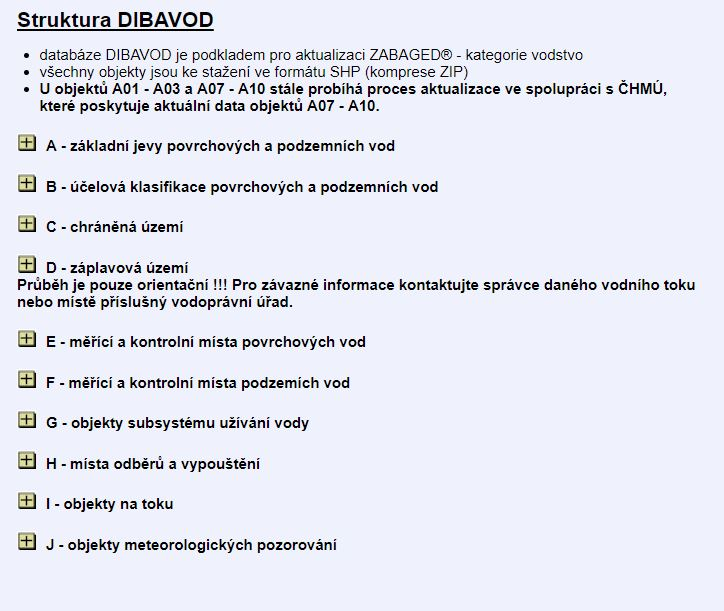
\includegraphics[width=13cm]{pictures/dibavod.jpg}
	\caption{Struktura dat DIBAVOD}
\end{figure}

\subsection{OpenStreetMap}
OpenStreetMap je projekt, jehož cílem je tvorba volně dostupných geografických dat a následně jejich vizualizace do podoby silniční mapy, uliční mapy měst atd. Tato vektorová data jsou poskytována pod licencí Open Database Licence. \\
\\
Jedná se o taková zdrojová data, která může kdokoliv upravit. Díky tomu se na tvorbě může podílet v podstatě kdokoliv, v současné době navíc existují i pluginy, které umožňují stáhnutí OMS do Garminu či smartphonů. 

\begin{figure}[h!]
	\centering
	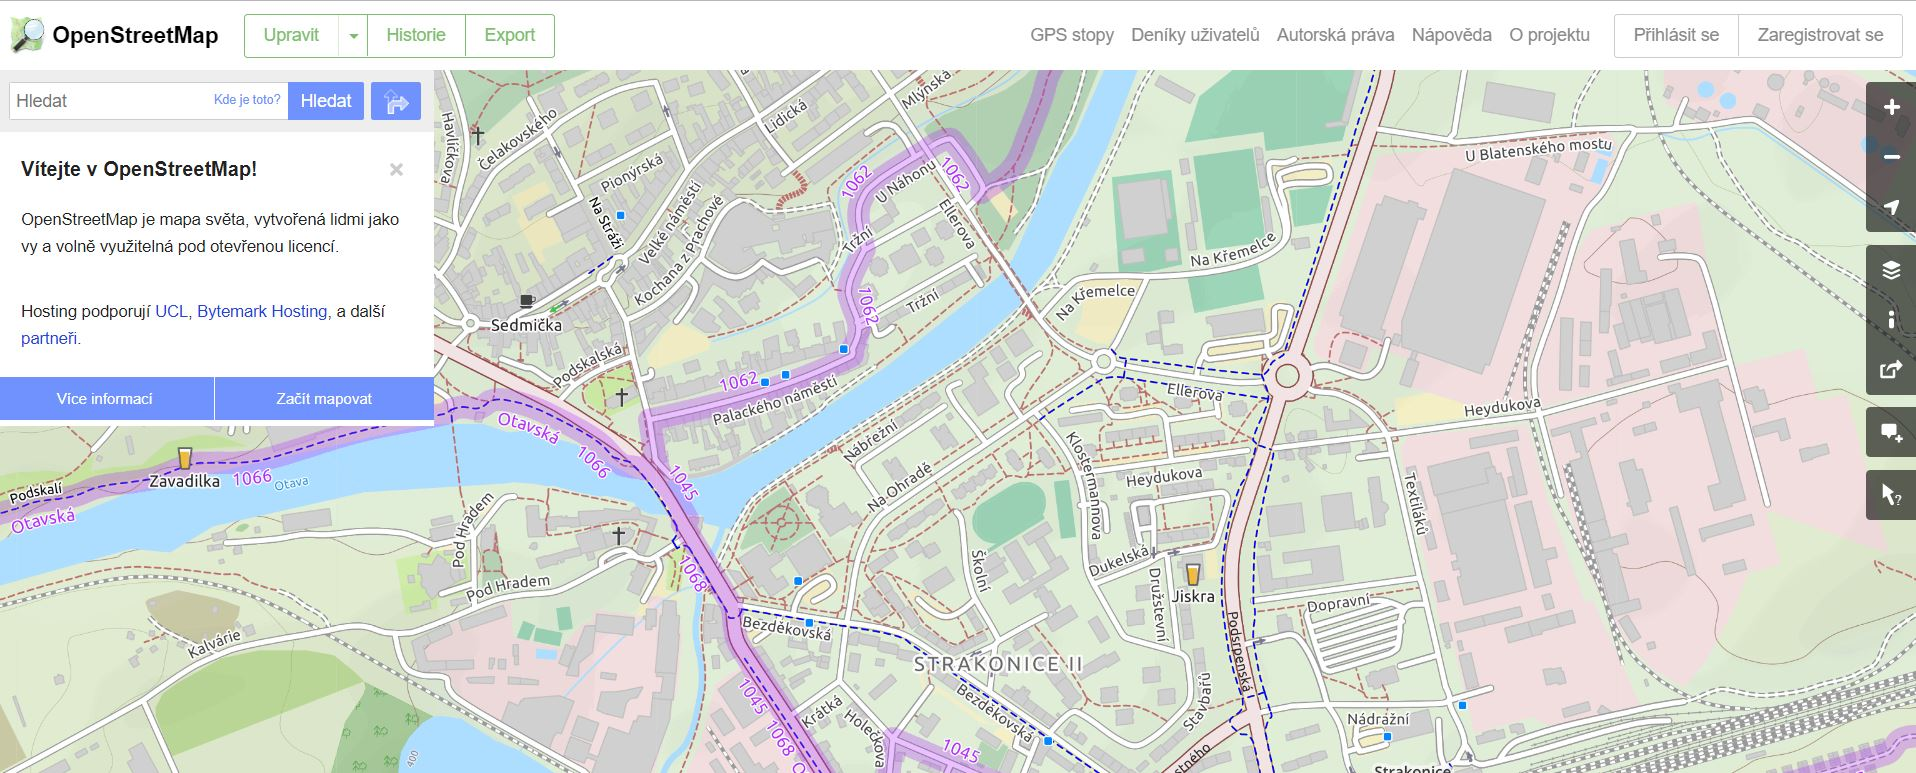
\includegraphics[width=14cm]{pictures/osm.jpg}
	\caption{Ukázka OpenStreetMap pro část Strakonic}
\end{figure}


\subsection{ArcČR 500}
ArcČR 500 je digitální vektorová geografická databáze České republiky. Data vznikla ve spolupráci ARCDATA Praha, s.r.o., Zeměměřického úřadu a Českého statistického úřadu. Data jsou pro uživatele k dispozici zdarma. \\
\\
Data lze rozdělit do tří hlavních složek - Administrativní členění, Geografické prvky a Klady a sítě. Pro projekt byly zahrnuty jen určité vrstvy z kategorie Geografické prvky a Administrativní členění. 

\begin{figure}[h!]
	\centering
	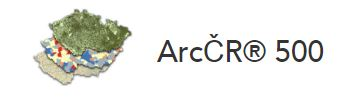
\includegraphics[width=8cm]{pictures/arccr.jpg}
	\caption{Logo ArcČR 500}
\end{figure}

\subsection{AOPK ČR}
Agentura Ochrany Přírody a Krajiny ČR nabízí datové sady týkající se národně i mezinárodně chráněných územích či druzích, památných stromech, biotopech, rezervacích, geoparcích či mokřadech. Data jsou v souřadnicovém systému WGS84 a organizace nabízí řadu formátů, ve kterých lze data stáhnout.\\
\\
Agentura spadá pod Ministerstvo životního prostředí a v roce 2017 získala ocenění na evropské konferenci INSPIRE ve Štrasburku. 

\begin{figure}[h!]
	\centering
	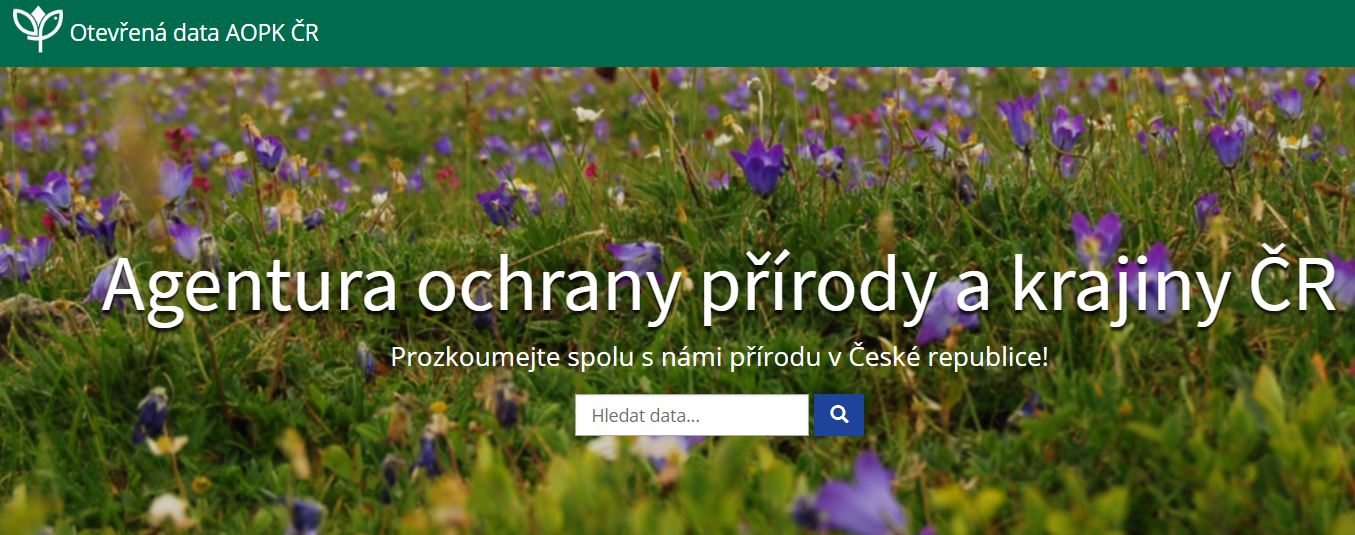
\includegraphics[width=12cm]{pictures/aopk.jpg}
	\caption{Agentura ochrany přírody a krajiny ČR}
\end{figure}


\subsection{ČSÚ}
Český statistický úřad je ústřední orgán státní správy České republiky. Je nezávislý na vládě a politických stranách. ČSÚ zajišťuje zpracování a zveřejňování údajů, sestavuje souhrnné statistické charakteristiky vývoje národního hospodářství, zpracovává analýzy, zároveň shromažďuje i zahraniční statistické informace a jednou za 10 let provádí Sčítání lidu. \\
\\
Všechna data a informace jsou na serveru zdarma pro státní správu i běžného užiivatele. Data jsou většinou k dispozici ve dvou formátech - ve formátu XML a CVS. Jedním ze známých produktů ČSÚ jsou také výsledky voleb.

\begin{figure}[h!]
	\centering
	
\includegraphics[width=12cm]{pictures/csu.jpg}
	\caption{Logo Českého statistického úřadu}
\end{figure}


\section{Software}
\subsection{QGIS}
Tvorba databáze a prostorových dotazů probíhala ve frameworku QGIS. Aplikace QGIS je velmi podobná programu ArcGIS od společnosti ESRI, velkou výhodou však je to, že se jedná o multiplatformní program, který je zcela zdarma. V dnešní době je velmi rozšířen a existuje mnoho zásuvných modulů (pluginů), které mají v sobě naimplementovány často používané funkce.\\
\\

\begin{figure}[h!]
	\centering
	
\includegraphics[width=5cm]{pictures/qgis.png}
	\caption{QGIS}
\end{figure}

Ve frameworku QGIS má uživatel možnost vytvářet, editovat či čistě jen prohlížet rastrová a vektorová geodata. V rámci programu je možné provádět prostorové a atributové dotazy. Zároveň je možná práce s webovými službami OGC. Uživatel má také možnost importovat data s oddělenými hodnotami (př. CSV) či připojit tabulková data.\\
\\

\begin{figure}[h!]
	\centering
	
\includegraphics[width=8cm]{pictures/qgis.jpg}
	\caption{QGIS}
\end{figure}

\subsection{PostGIS}
PostGIS je open source program, který je nadstavbou objektově relačního databázového systému PostgreSQL, jenž rozšiřuje podporu systému o geografické objekty. PostGIS podporuje mimo QGIS např. Mapnik nebo Quantum GIS. Tato nadstavba umožňuje manipulovat a analyzovat geodata za pomoci dotazovacího jazyka SQL. 

\begin{figure}[h!]
	\centering
	
\includegraphics[width=10cm]{pictures/postgis.png}
	\caption{PostGIS}
\end{figure}


\section{Praktická část}
\subsection{Databáze}
Nejprve bylo nutné se připojit na server, na němž bude uložena vytvořená geodatabáze. Připojení může probíhat prostřednictvím příkazové řádky nebo přes konzoli v prostředí QGIS. Databáze pro tento projekt byla vytvářena přes konzoli. 

\begin{figure}[h!]
	\centering
	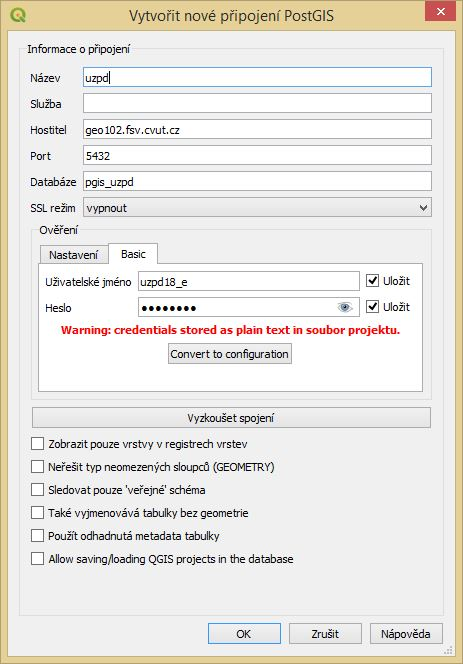
\includegraphics[width=6cm]{pictures/pripojeni.jpg}
	\caption{Připojení databáze}
\end{figure}

Import jednotlivých vrstev probíhal také přes konzoli, kde bylo nutné zvolit vrstvu, kterou nahráváme, schéma, do nějž bude vrstva nahrána, zvolit sloupec s geometrií a zejména nastavit souřadnicový systém vrstvy. Data ze stránek AOPK byla v systému WGS84. Všechny vrstvy v databázi byly nahrány v systému JTSK, data z AOPK bylo tedy nutné transformovat, což dle obrázku šlo velmi snadno.


\begin{figure}[h!]
	\centering
	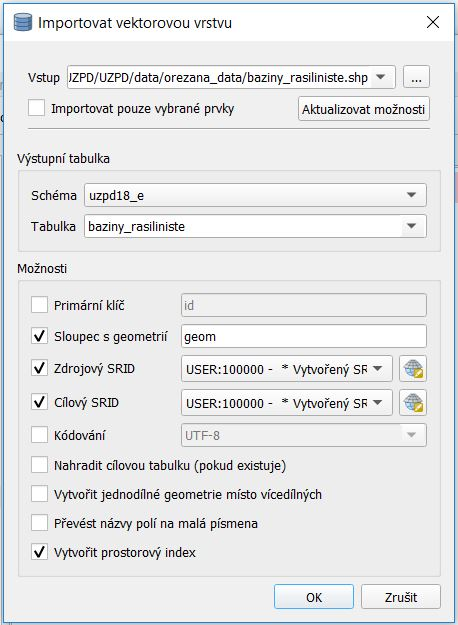
\includegraphics[width=6cm]{pictures/import.jpg}
	\caption{Import vrstev}
\end{figure}


Data jsou v konzolové aplikace přehledná, lze si po rozkliknutí dané vrstvy zobrazit informace o tabulce, samotnou tabulku s daty či náhled dat. Pro následnou tvorbu SQL dotazů poté stačí rozkliknout jen ikonu SQL okno.

\begin{figure}[h!]
	\centering
	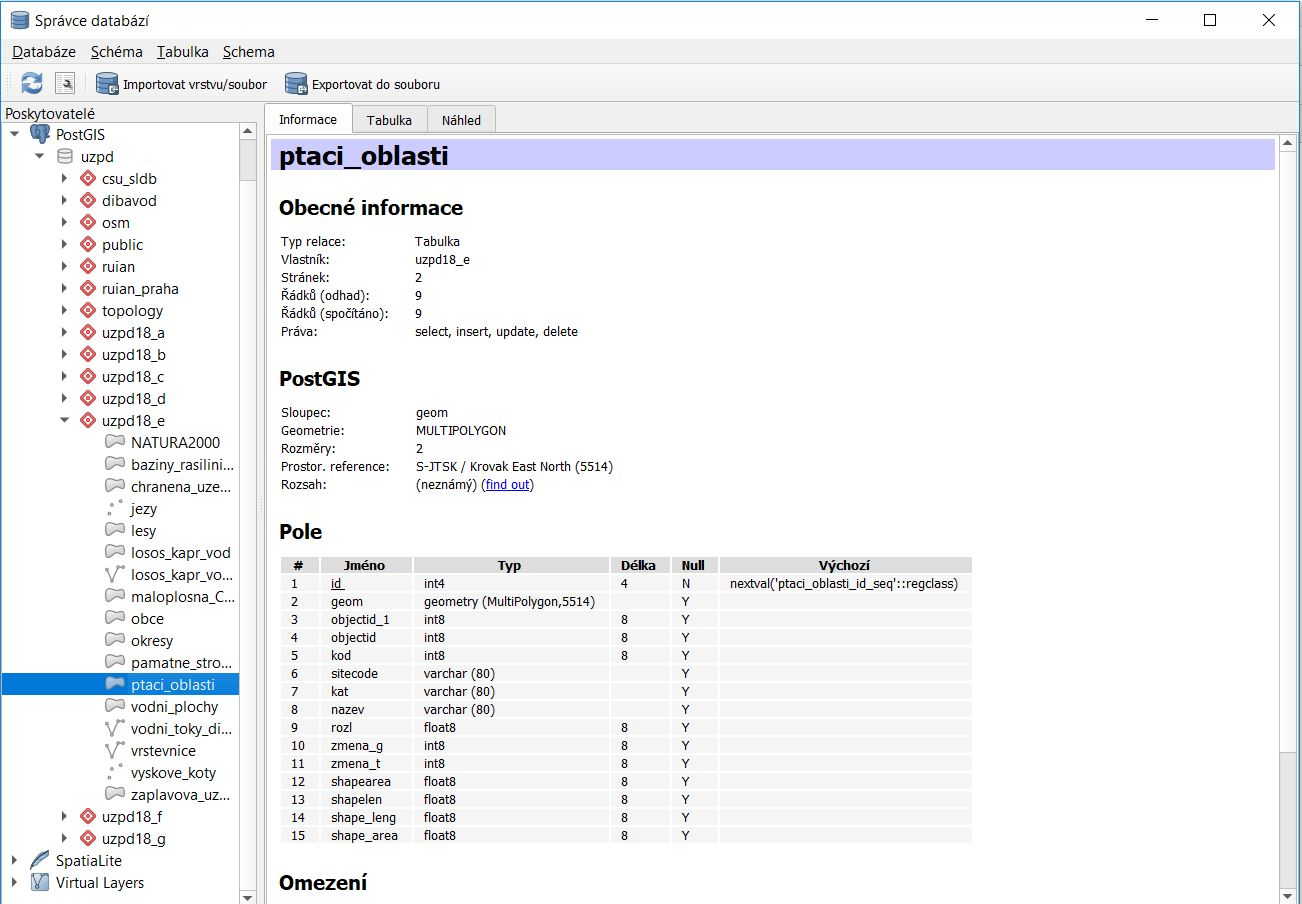
\includegraphics[width=12cm]{pictures/vzhled.jpg}
	\caption{Vzhled a schéma databáze}
\end{figure}

\subsection{Validace dat}
Stažená data však nemusí být validní, což znamená, že geometrie dat není topologicky správná. Pro zjištění a opravu byly použity tři funkce. Funkce ST\_IsValid je taková funkce, která pro jednotlivé záznamy tabulky vrací TRUE (v případě, že geometrie je validní) nebo FALSE (geometrie není validní). Funkce ST\_IsValidReason vrací důvod, proč není geometrie validní. Následně funkce ST\_MakeValid ze zadané geometrie vytvoří novou topologicky správnou geometrii.\\
\\
\begin{figure}[h!]
	\centering
	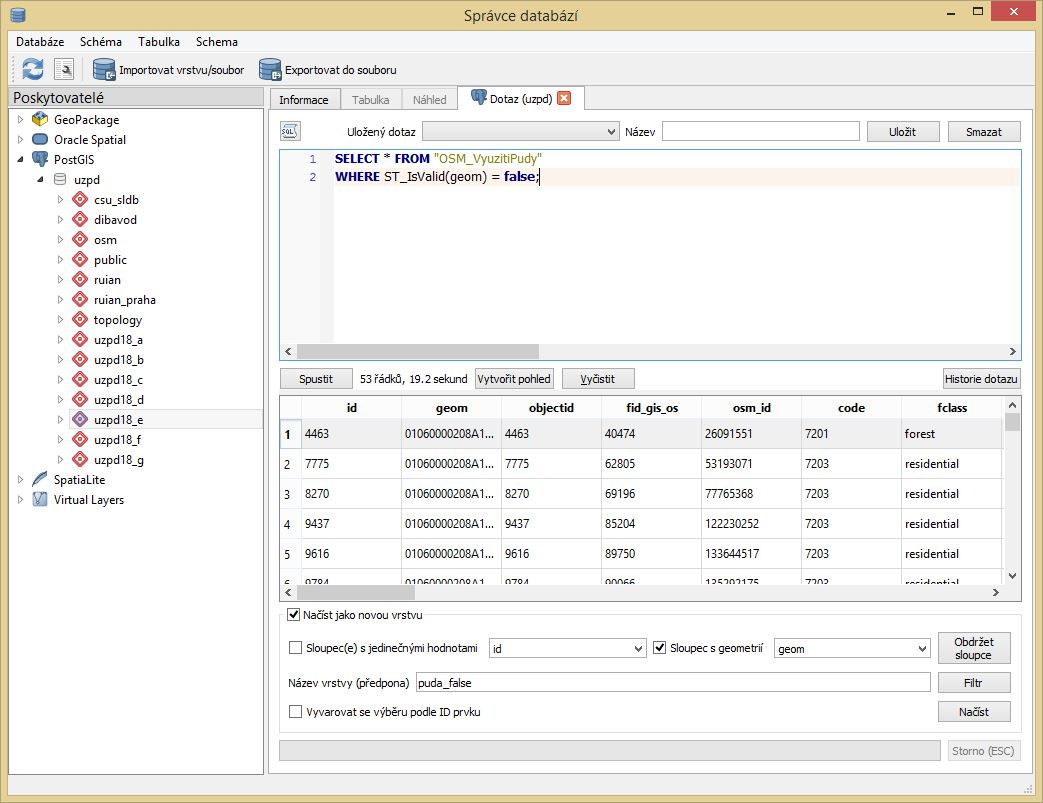
\includegraphics[width=8cm]{pictures/validace.jpg}
	\caption{Příklad zjišťování chyby}
\end{figure}

Na obrázku č. 12 lze vidět použití funkce pro zjištění důvodu chyby. Příkaz navrátí id a název chyby, v tomto případě navrátil "ID, Ring Self - Intersection". Tuto chybu odstraníme následujícím příkazem: \\

\begin{figure}[h!]
	\centering
	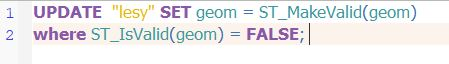
\includegraphics[width=8cm]{pictures/oprava_val.jpg}
	\caption{Příkaz pro opravení chybné topologie}
\end{figure}

Na obrázku č. 13 je příkaz pro opravu dat. Tato funkce přepíše geometrii pro záznamy s nevalidní geometrií a novou geometrii získanou funkcí ST\_MakeValid.\\
\\

Veškeré příkazy pro zjištění validace včetně výsledků lze nalézt v přiloženém souboru davka.sql. Vrstvy, které se v současné době nachází v databázi, jsou validní.\\
\\
\clearpage
\subsection{Vrstvy}
Pro zadané téma bylo použito několik vrstev z různých zdrojů. Níže jsou jednolivé vrstvy stručně popsány.

\subsubsection{CSU\_statistika\_obyvatel}
CSU\_statistika\_obyvatel je tabulka s daty staženými ze stránek Českého statistického úřadu. 

\subsubsection{NATURA2000}
Jedná se o polygonovou vektorovou vrstvu. Zahrnuje hranice evropsky významných lokalit vymezených v rámci soustavy Natura 2000 a určených k ochraně přírodních stanovišť nebo populací druhů dle platného nařízení vlády, kterým se stanoví národní seznam evropsky významných lokalit, volně žijících živočichů a planě rostoucích rostlin. Data pochází ze stránek AOPK a jsou v systému WGS-84. Geometrie prvků je Multipolygon.

\subsubsection{OSM\_NabozenskeObjekty}
V této vrstvě se nachází náboženské objekty v Jihočeském kraji z dat OSM. Geometrie prvků je Multipoint. Vrstva obsahuje objekty různých náboženských vyznání. Ve zvoleném zájmovém území se nachází křesťanské a židovské budovy. U některých prvků je křesťanství ještě rozděleno, zda se jedná o protestantské či katolické. Tato skutečnost může být pro uživatele matoucí, neboť nejsou jednotně definovány hodnoty, kterých může kolonka vyznání nabývat.

\subsubsection{OSM\_StromyVrchy}
Geometrie prvků této vrstvy je Multipoint. Data jsou z OpenStreetMap a lze je rozdělit do 6 hlavních složek, a to na prameny (případně studánky), útesy (skály), vrcholy, jeskyně, pláže a stromy.

\subsubsection{OSM\_VyuzitiPudy}
Geometrie prvků je Multipolygon. Kategorie pro jednotlivá data jsou louky, rekreační střediska (kempy), území zemědělských družstev, vojenská území, podrosty, průmyslové oblasti, komerční oblasti (výstaviště), vřesoviště, přírodní rezervace, travnaté oblasti, hřbitovy, parky, obydlí, sady, lesy, lomy, osady a maloobchody. Tato data pochází z OpenStreetMap.


\subsubsection{baziny\_rasiliniste}
Vrstva pochází z dat ArcČR 500. Data byla v systému S-JTSK. Geometrie prvků je Multipolygon. Ve vrstvě jsou pouze bažiny a rašeliniště, jejichž plocha je větší než 30 ha. Data nabývají hodnot 1 (bažiny) nebo 2 (rašeliniště).

\subsubsection{chranena\_uzemi}
Geometrie prvků je Multipolygon. Vrstva pochází ze zdroje ArcČR 500. Data nabývají hodnot 1 (Národní park) či 2 (Chráněná krajinná oblast).

\subsubsection{jezy}
Geometrie prvků je Multipoint. Vrstva pochází ze stránek DIBAVOD z kategorie objekty na toku. Data byla v systému S-JTSK.

\subsubsection{lesy}
Tato vrstva pochází ze stránek ArcČR 500. Geometrie prvků je Multipolygon. Vrstva obsahuje lesní plochy větší než 30 ha. 

\subsubsection{losos\_kapr\_oblasti}
Vrstva losos\_kapr\_oblasti byla stažena ze stránek DIBAVOD. Geometrie prvků je Multipolygon. Jedná se o oblasti povodí povrchové vody, které jsou či se stanou vhodné pro život a reprodukci původních druhů ryb a dalších vodních živočichů. Data lze rozdělit do dvou kategorií - lososové vody (vhodné pro život ryb lososovitých a lipana) a kaprové vody (vhodné pro život ryb kaprovitých nebo jiných druhů, jako je štika, okoun a úhoř). 


\subsubsection{losos\_kapr\_toky}
Geometrie prvků je Multilinestring. Data pochází ze stránek DIBAVOD a 2 hlavní kategorie jsou stejné jako u výše zmíněné polygonové vrstvy losos\_kapr\_oblasti.


\subsubsection{maloplosna\_CHU\_AOPK}
Data pro tuto vrstvu byla stažena ze stránek AOPK v systému WGS-84. Geometrie prvků je Multipolygon. Vrstva obsahuje hranice vyhlášených maloplošných zvláště chráněných území (národní přírodní rezervace, národní přírodní památky, přírodní rezervace a přírodní památky) a jejich ochranných pásem. Data se mohou navzájem překrývat. 


\subsubsection{obce}
Geometrie prvků je Multipolygon. Jedná se o vrstvu obsahující všechny obce v Jihočeském kraji. Data pochází ze zdroje ArcČR 500 a jsou v systému S-JTSK.

\subsubsection{okresy}
Geometrie prvků je Multipolygon. Jedná se o vrstvu obsahující všechny okresy v Jihočeském kraji. Data pochází ze zdroje ArcČR 500 a jsou v systému S-JTSK.

\subsubsection{pamatne\_stromy}
Vrstva pochází ze stránek AOPK a je v systému WGS-84. Zahrnuje obejkty, které byly vyhlášeny jako památné stromy. Data obsahují jednoduché prvky - singlepart features. Dle sloupce typ lze jednotlivé prvky rozdělit na bodové (1 - památný strom), liniové (2 - stromořadí či alej) a plošné (3 - skupina stromů či arboretum).

\subsubsection{ptaci\_oblasti}
Vrstva ptaci\_oblasti obsahuje hranice ptačích oblastí vymezených v rámci soustavy Natura 2000 a určených k ochraně ptačích druhů dle platných nařízení vlády, kterými se vymezují ptačí oblasti. Geometrie prvků je Multipolygon a data jsou v systému WGS-84. 

\subsubsection{vodni\_plochy}
Vrstva vodni\_plochy pochází z dat ArcČR 500. Geometrie prvků je Multipolygon. Data obsahují vodní nádrže, rybníky a jezera s plochou větší než 15 ha. Typ vodní plochy je kategorizován sloupcem typ, kde 1 - vodní nádrž, 2 - rybník a 3 - jezero. 

\subsubsection{vodni\_toky\_dibavod}
Vodní toky pochází ze stránek DIBAVOD. Geometrie prvků je Multilinestring. Byla vybrána vrstva vodních toků s hrubými úseky. Data byla v systému S-JTSK. 


\subsubsection{vyskove\_koty}
Výškové kóty lze najít ve vrstvě vyskove\_koty. Geometrie prvků je Multipoint a data pochází z ArcČR 500. 

\subsubsection{zaplavova\_uzemi\_20}
Vrstva znázorňuje záplavová území dvacetileté vody. Geometrie prvků je Multipolygon. Data pochází ze stránek DIBAVOD a jejich průběh je pouze orientační, neboť se nedá zahrnout všechny aktuální aspekty záplav. Z toho důvodu je při potřebě aktuálních dat nutné kontaktovat správce daného vodního toku. Pro akademické účely však postačí přibližná data.

\section{Dotazy}

\subsection{Atributové dotazy}
Atribut popisuje negeometrickou vlastnost entity. Atributové dotazy lze popsat tak, že se dotazují na atributy geografických dat. Lze je uskutečnit různými způsoby, např. identifikací jednotlivého objektu na základě jeho jména, označení či jiného atributu či vyhledáním všech objektů splňujících intervalové či logické podmínky jednoho nebo více atributů. \\
\\
V rámci projektu bylo vytvořeno několik atributových dotazů. Při tvorbě dotazů byla snaha pokrýt všechny operátory, které byly vyzkoušeny v rámci cvičení. Veškeré dotazy lze najít v soubor davka.sql, zde je uvedeno pouze pár příkladů. Při tvorbě dotazů neexistuje jediné správné řešení, možností, jak se dostat ke správnému výsledku za pomoci různých funkcí je několik. U některých dotazů se tedy objevují alternativní řešení, která vedou také ke správným výsledkům. \\
\\

\begin{figure}[h!]
	\centering
	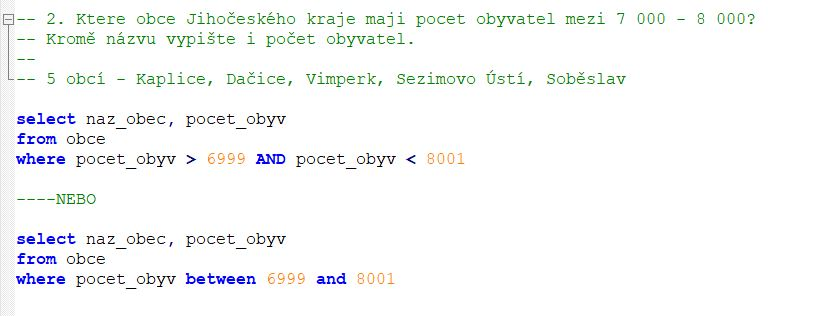
\includegraphics[width=15cm]{pictures/at1.jpg}
\end{figure}

\begin{figure}[h!]
	\centering
	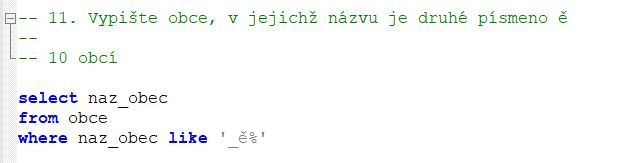
\includegraphics[width=15cm]{pictures/at2.jpg}
\end{figure}

\begin{figure}[h!]
	\centering
	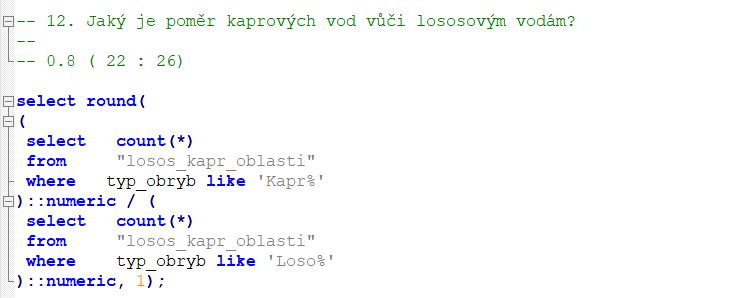
\includegraphics[width=15cm]{pictures/at3.jpg}
\end{figure}

\subsection{Prostorové dotazy}
Při použití prostorových dotazů zajímá uživatele prostorová složka dat. Dotazy se mohou týkat určité vzdálenosti, hraničení, křížení apod. Jsou tedy zaměřené na prostorové vlastnosti a vztahy geografických dat. \\
\\
Mezi nejčastější funkce používané v prostorových dotazech patří průnik (data se překrývají), dotyk (linií či bodem), obsažení v některé oblasti či prvku, identičnost či nacházení se v určité vzdálenosti od daného prvku či oblasti. 

\begin{figure}[h!]
	\centering
	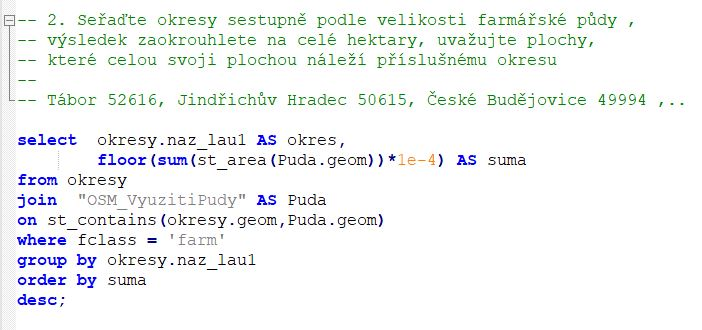
\includegraphics[width=15cm]{pictures/pd1.jpg}
\end{figure}

\begin{figure}[h!]
	\centering
	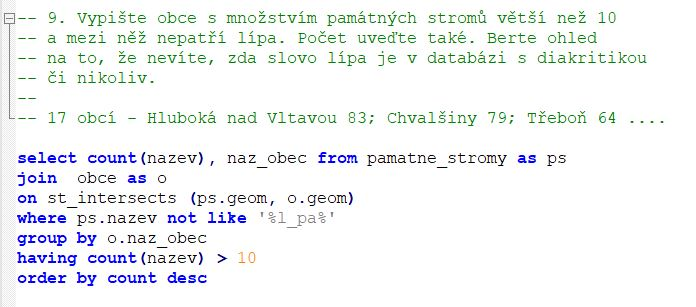
\includegraphics[width=15cm]{pictures/pd3.jpg}
\end{figure}

\clearpage

\begin{figure}[h!]
	\centering
	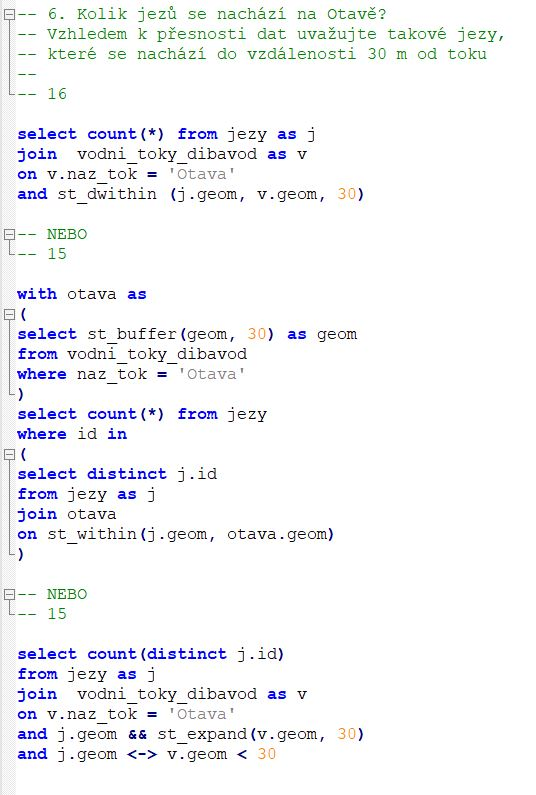
\includegraphics[width=15cm]{pictures/pd2.jpg}
\end{figure}

\clearpage 
\begin{figure}[h!]
	\centering
	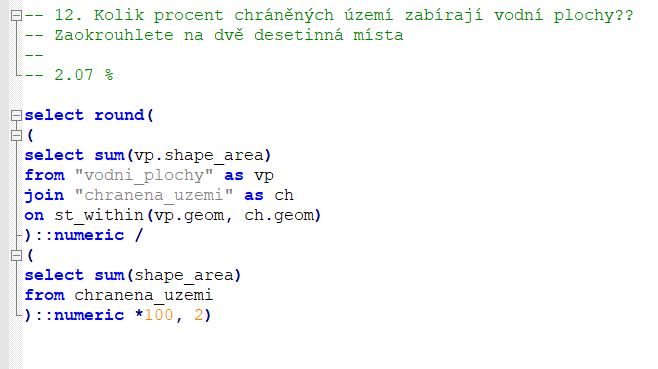
\includegraphics[width=15cm]{pictures/pd4.jpg}
\end{figure}

V rámci dokumentace nebyly zveřejňovány všechny vytvořené dotazy. Ty lze nalézt v souboru davka.sql. 


\clearpage
\section{Závěr}
Hlavním cílem tohoto projektu bylo vytvoření vlastní databáze s vlastním výběrem vrstev, nad nimiž budou následně volány atributové a prostorové dotazy. Původním plánem bylo vytvoření databáze pro okres Strakonice, po upozornění na množství dat bylo zájmové území rozšířeno na celý Jihočeský kraj. Databáze včetně vrstev byla úspěšně vytvořena a dotazy vrací správné výsledky.\\
\\
V rámci výběru jednotlivých vrstev byly prozkoumány veřejně dostupné zdroje. Velmi kladně hodnotí autoři stránky AOPK, která je velmi překvapila. stránka je přehledná a srozumitelná. Pozitivní hodnocení mají i data ArcČR 500, která mají perfektně vytvořená metadata. Data z ČSÚ byla použita z toho důvodu, aby bylo v rámci projektu vyzkoušeno také připojování tabulek. \\
\\
Co se týče dotazů, byly vytvářeny tak, aby v souboru davka.sql byly postupně složitější. Jejich obtížnost se tedy postupně zvyšuje. Navíc byl kladen důraz i na to, aby byla použita většina operátorů a funkcí. \\
\\
Obecně hodnotí autoři projekt za přínosný. Nabyli nové znalosti a zkušenosti týkající se databází a PostGISu. 




\clearpage
\section{Reference}

\begin{enumerate}
\item  Agentura ochrany přírody a krajiny ČR [online][cit. 5.1.2019]. \\
Dostupné z: http://gis-aopkcr.opendata.arcgis.com/  \\

\item  Oddělení geografických informačních systémů a kartografie [online][cit. 5.1.2019]. \\
Dostupné z: http://www.dibavod.cz/index.php?id=27  \\

\item  ArcData Praha [online][cit. 5.1.2019]. \\
Dostupné z: https://www.arcdata.cz/produkty/geograficka-data/arccr-500  \\

\item  Český statistický úřad [online][cit. 5.1.2019]. \\
Dostupné z: https://www.czso.cz/ \\

\item OpenStreetMap [online][cit. 5.1.2019]. \\
Dostupné z: https://download.geofabrik.de/europe/czech-republic.html?fbclid=IwAR3wKATBPMRuy7KgqaJm1pj\_sYjYVF7K2C8In\_tCOrPE29hJoFblm5TdWfc \\

\item LANDA, Martin. Úvod do zpracování prostorových dat [online][cit. 28.1.2019]. \\
Dostupné z: http://geo.fsv.cvut.cz/~gin/uzpd/\\

\item PACINA, Jan. Atributové a prostorové dotazy [online][cit. 28.1.2019]. \\
Dostupné z: http://gis.fzp.ujep.cz/files/3.Prednaska.pdf \\

\item GISMentors [online][cit. 28.1.2019]. \\
Dostupné z: http://gismentors.cz/ \\

\item PostGIS 2.5.2dev Manual [online][cit. 28.1.2019]. \\
Dostupné z: http://postgis.net/docs/ \\

\end{enumerate}
\end{document}



 